\begin{figure}[!htbp]
	\centering
	\begin{tabular}{cc}
		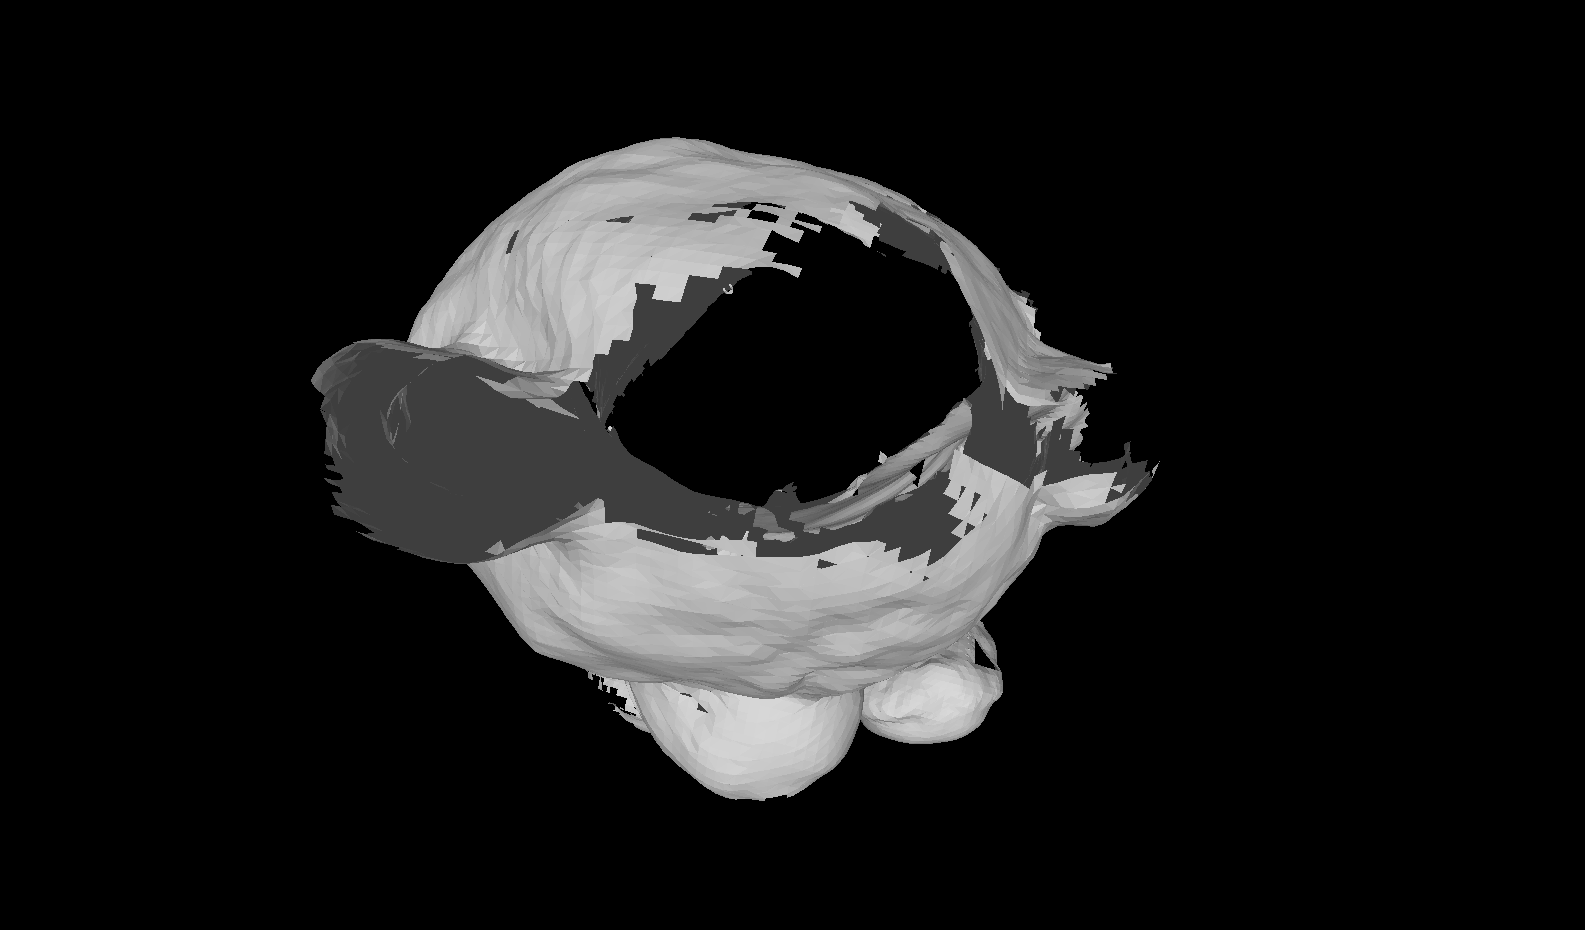
\includegraphics[width=.3\linewidth]{figures/object_recon/gappy/one_scene00.png}&
    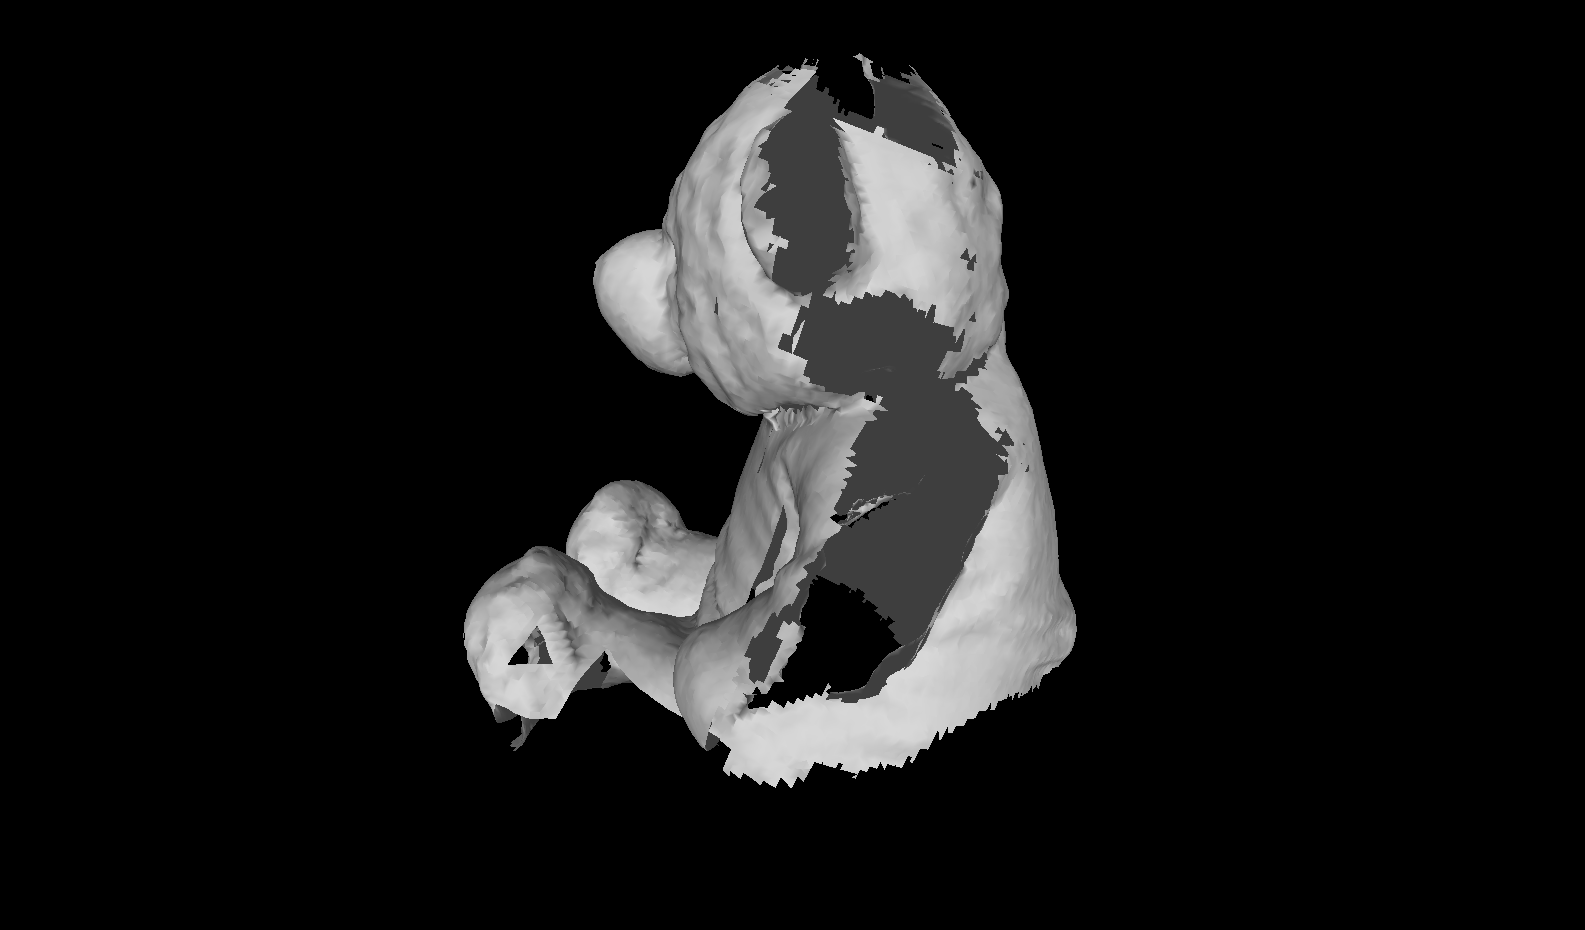
\includegraphics[width=.3\linewidth]{figures/object_recon/gappy/one_scene01.png}\\
    (a) & (b) \\
		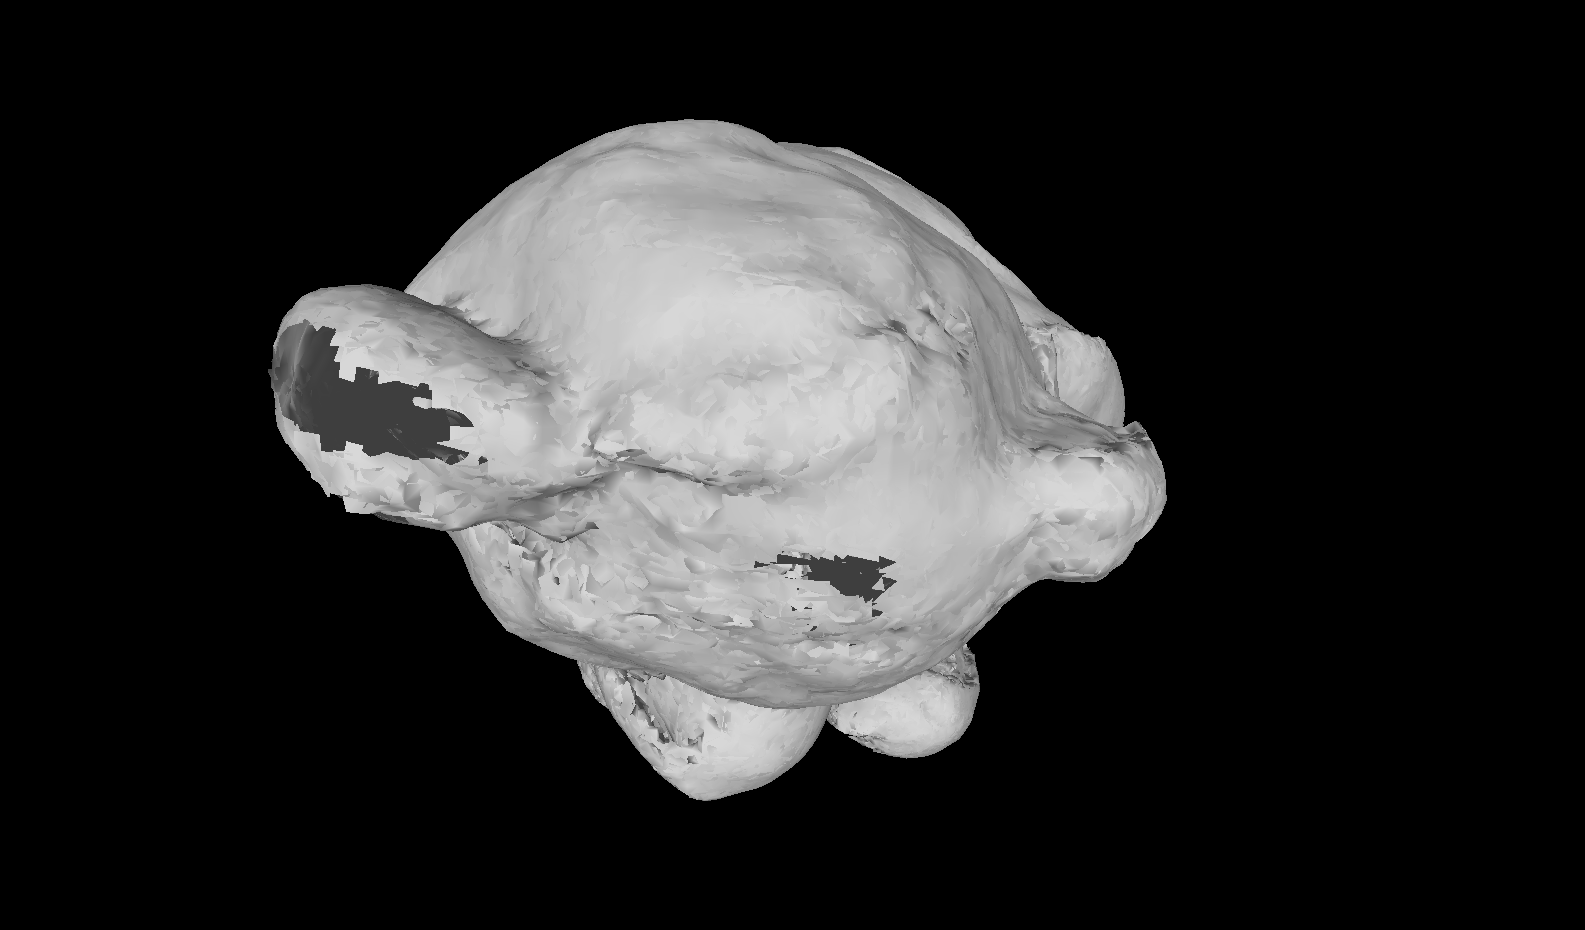
\includegraphics[width=.3\linewidth]{figures/object_recon/gappy/multi_scene00.png}&
    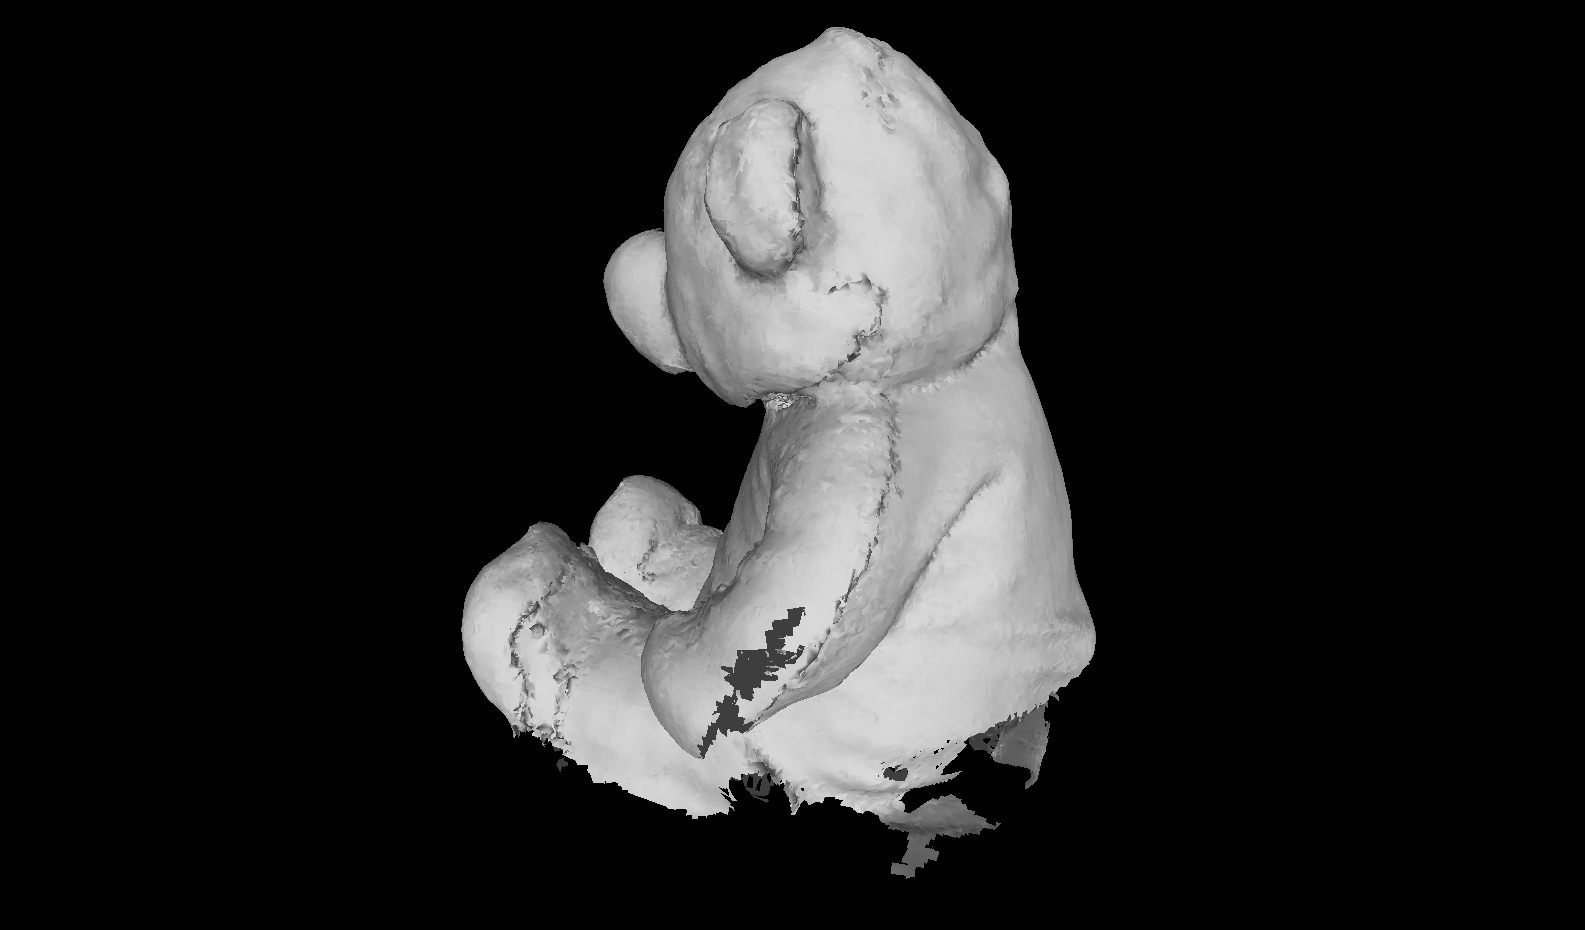
\includegraphics[width=.3\linewidth]{figures/object_recon/gappy/multi_scene01.png}\\
    (c) & (d)\\
	\end{tabular}
  \caption[Probabilistic Object Reconstruction Qualitative Results V]
  {
    Teddy reconstruction with InfiniTAM (a, b) versus the system proposed in this 
    work (c, d).
  }
~\label{figure:probobj_gappy_teddy}
\end{figure}